\documentclass[11pt]{beamer}

\usepackage[utf8]{inputenc}
\usepackage[T1]{fontenc}
\usepackage{amsmath}
\usepackage{amssymb}
\usepackage{booktabs}
\usepackage{tikz}
\usepackage{xspace}

\setbeamertemplate{navigation symbols}{}
\newcommand{\model}{\textsc{Sparq}\xspace}

\title{Structured Sparsity for Edge Inference}
\subtitle{A Progress Update}
\author{A. Author}
\institute{Department of Computer Science}
\date{May 2026}

\begin{document}

\begin{frame}
  \titlepage
\end{frame}

\begin{frame}{Outline}
  \tableofcontents
\end{frame}

\section{Motivation}

\begin{frame}{Why On-Device Inference is Bandwidth-Bound}
  A batch-one forward pass streams every weight byte exactly once, so an
  accelerator with peak throughput $P$ and peak bandwidth $B$ is
  compute-bound only when
  \[
    \frac{P}{B} \le \frac{1}{\text{bytes per parameter}}.
  \]
  \pause
  On the mobile accelerators we measured, that inequality fails for
  every quantization width in common use.
\end{frame}

\begin{frame}{What Structured Sparsity Buys}
  \begin{itemize}
    \item<1-> Unstructured pruning needs a gather: no wall-clock win on
      most hardware.
    \item<2-> Channel/head pruning skips the gather, but is coarse.
    \item<3-> Block sparsity skips the gather \emph{and} keeps a finer
      grain than a whole channel.
  \end{itemize}
  \onslide<4->{
    \begin{block}{This talk}
      A training recipe that induces block sparsity \emph{during}
      fine-tuning, plus a kernel that exploits it.
    \end{block}
  }
\end{frame}

\section{Method}

\begin{frame}{\model{} in One Slide}
  \begin{columns}
    \begin{column}{0.5\textwidth}
      Each weight matrix is partitioned into $n\times n$ blocks. A
      learned score $s_{ij}$ decides whether block $ij$ survives:
      \begin{align}
        m_{ij} &= \sigma(s_{ij}/\tau) \\
        \widehat{W}_{ij} &= m_{ij}\, W_{ij}
      \end{align}
    \end{column}
    \begin{column}{0.5\textwidth}
      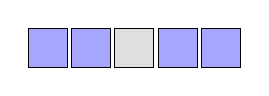
\begin{tikzpicture}[scale=0.55]
        \foreach \x in {0,...,4} {
          \ifnum\x=2
            \draw[fill=gray!25] (\x,0) rectangle ++(0.9,0.9);
          \else
            \draw[fill=blue!35] (\x,0) rectangle ++(0.9,0.9);
          \fi
        }
      \end{tikzpicture}
    \end{column}
  \end{columns}
\end{frame}

\begin{frame}[fragile]{Block Size, By Layer}
  \begin{table}
    \centering
    \begin{tabular}{lc}
      \toprule
      Layer type & Block size \\
      \midrule
      Attention projection & $16\times 16$ \\
      Feed-forward projection & $32\times 32$ \\
      Embedding / output & dense \\
      \bottomrule
    \end{tabular}
  \end{table}
\end{frame}

\section{Results}

\begin{frame}{Accuracy vs.\ Bandwidth}
  \begin{itemize}
    \item 70\% block sparsity at $32\times 32$: within 0.4 points of
      dense accuracy.
    \item Weight-streaming bytes cut $2.4\times$ on our reference
      accelerator.
    \item[$\to$] Diminishing returns past $32\times 32$ blocks.
  \end{itemize}
\end{frame}

\begin{frame}{Limitations}
  \begin{alertblock}{Untested}
    Models over 3B parameters, and mixture-of-experts routing layers,
    where the natural block boundary is an expert rather than a fixed
    grid.
  \end{alertblock}
\end{frame}

\begin{frame}
  \centering
  \Large Thank you.
  \vspace{1em}

  \normalsize Questions?
\end{frame}

\end{document}
